\subsection{Relación 1. Integración Numérica}
\setcounter{ejercicio}{8}

\begin{ejercicio}\label{ej:2.1.9}
    Se considera la siguiente fórmula de integración numérica:
    \begin{equation*}
        \int_{-1}^{1} f(x) dx \approx \alpha_0 f(-1) + \alpha_1 f(0) + \alpha_2 f(1).
    \end{equation*}
    \begin{enumerate}
        \item Halle de tres formas distintas los valores $\alpha_i \in \mathbb{R}$, $i = 0, 1, 2$ para que dicha fórmula sea de tipo interpolatorio en $\bb{P}_2$.
        
        \begin{enumerate}
            \item \ul{Integración de los polinomios fundamentales de Lagrange:}
            \begin{align*}
                \alpha_0 &= \int_{-1}^{1} \ell_0(x) dx = \int_{-1}^{1} \frac{(x - 0)(x - 1)}{(-1 - 0)(-1 - 1)} dx = \int_{-1}^{1} \frac{x^2 - x}{2} dx = \dfrac{1}{2} \left[ \frac{x^3}{3} - \frac{x^2}{2} \right]_{-1}^{1} =\\&= \dfrac{1}{2} \left( \frac{1}{3} - \frac{1}{2} + \frac{1}{3} + \frac{1}{2} \right) = \dfrac{1}{3},\\
                \alpha_1 &= \int_{-1}^{1} \ell_1(x) dx = \int_{-1}^{1} \frac{(x + 1)(x - 1)}{(0 + 1)(0 - 1)} dx = \int_{-1}^{1} -x^2 + 1 dx = 2\cdot \int_{0}^{1} 1-x^2 dx =\\&= 2\cdot \left[ x - \frac{x^3}{3} \right]_{0}^{1} = 2\cdot \left( 1 - \frac{1}{3} \right) = \dfrac{4}{3},\\
                \alpha_2 &= \int_{-1}^{1} \ell_2(x) dx = \int_{-1}^{1} \frac{(x + 1)(x - 0)}{(1 + 1)(1 - 0)} dx = \int_{-1}^{1} \frac{x^2 + x}{2} dx = \dfrac{1}{2} \left[ \frac{x^3}{3} + \frac{x^2}{2} \right]_{-1}^{1} =\\&= \dfrac{1}{2} \left( \frac{1}{3} + \frac{1}{2} + \frac{1}{3} - \frac{1}{2} \right) = \dfrac{1}{3}.
            \end{align*}

            \item \ul{Imponiendo exactitud en $\bb{P}_2$:}
            \begin{align*}
                2 = \int_{-1}^{1} 1 dx &= \alpha_0 + \alpha_1 + \alpha_2,\\
                0 = \int_{-1}^{1} x dx &= -\alpha_0 + \alpha_2,\\
                \nicefrac{2}{3} = \int_{-1}^{1} x^2 dx &= \alpha_0 + \alpha_2
            \end{align*}

            Sistituyendo la tercera ecuación en la primera:
            \begin{align*}
                2 &= \alpha_1 + \frac{2}{3}\Longrightarrow \alpha_1 = 2 - \frac{2}{3} = \frac{4}{3}
            \end{align*}

            Sumando la segunda y la tercera, obtenemos:
            \begin{equation*}
                \alpha_2 = \frac{1}{3} = \alpha_0.
            \end{equation*}


            \item \ul{Integrando el polinomio de interpolación de Newton:}
            
            La tabla de diferencias divididas asociada a los nodos $-1$, $0$ y $1$ es:
            \begin{equation*}
                \begin{array}{c|cccc}
                    x_i & f[x_i] \\
                    \\
                    -1 & \mathbf{f(-1)} \\
                    && \mathbf{f(0)-f(-1)} \\
                    0 & f(0) & & \mathbf{\nicefrac{1}{2}(f(1)-2f(0)+f(-1))}\\
                    && f(1)-f(0)\\
                    1 & f(1)
                \end{array}
            \end{equation*}
            Por tanto, el polinomio de interpolación es:
            \begin{align*}
                p(x) &= f(-1) + \left(f(0)-f(-1)\right)(x+1) + \frac{1}{2}\left(f(1)-2f(0)+f(-1)\right)x(x+1)
                =\\&= f(-1)\left(1-1-x+\dfrac{x(x+1)}{2}\right) + f(0)\left(1+x-x(x+1)\right) + f(1)\left(\dfrac{x(x+1)}{2}\right)\\
                &= f(-1)\left(\dfrac{x(x-1)}{2}\right) + f(0)\left(1-x^2\right) + f(1)\left(\dfrac{x(x+1)}{2}\right).
            \end{align*}

            Empleando las integrales de los polinomios fundamentales de Lagrange ya vistos, tenemos:
            \begin{align*}
                \int_{-1}^{1} p(x) dx &= f(-1)\int_{-1}^{1} \dfrac{x(x-1)}{2} dx + f(0)\int_{-1}^{1} (1-x^2) dx + f(1)\int_{-1}^{1} \dfrac{x(x+1)}{2} dx =\\
                &= \dfrac{1}{3}\cdot f(-1) + \dfrac{4}{3}\cdot f(0) + \dfrac{1}{3}\cdot f(1).
            \end{align*}
        \end{enumerate}

        En cualquiera de los casos, obtenemos que:
        \begin{equation*}
            \alpha_0 = \alpha_2 = \frac{1}{3},\quad \alpha_1 = \frac{4}{3}.
        \end{equation*}

        La fórmula de integración numérica obtenida es:
        \begin{equation*}
            \int_{-1}^{1} f(x) dx \approx \frac{1}{3} f(-1) + \frac{4}{3} f(0) + \frac{1}{3} f(1).
        \end{equation*}
        \item Halle el grado de exactitud de la fórmula obtenida en el apartado anterior.
        
        Por construcción, sabemos que la fórmula es exacta en $\bb{P}_2$. Veamos si es exacta en $x^3$ y $x^4$:
        \begin{align*}
            \int_{-1}^{1} x^3 dx &= 0= -\frac{1}{3}+\frac{1}{3}\\
            \int_{-1}^{1} x^4 dx &= \frac{2}{5} \neq \frac{1}{3} + \frac{1}{3} = \frac{2}{3}.
        \end{align*}

        Por tanto, la fórmula es exacta en $\bb{P}_3$ y no es exacta en $\bb{P}_4$, por lo que su grado de exactitud es 3.
        \item Proporcione una fórmula de la forma propuesta que no sea de tipo interpolatorio en $\bb{P}_2$. Justifique la respuesta.
        
        Para ello, bassta encontrar valores de $\alpha_0$, $\alpha_1$ y $\alpha_2$ de forma que la fórmula no sea exacta en $\bb{P}_2$. Suponiendo por ejemeplo $\alpha_0 = \alpha_1 = \alpha_2 = 1$, tenemos:
        \begin{align*}
            \int_{-1}^{1} f(x) dx &\approx f(-1) + f(0) + f(1),\\
            \int_{-1}^{1} x^2 dx &= \frac{2}{3} \neq 1 + 1 + 1 = 3.
        \end{align*}
    \end{enumerate}
\end{ejercicio}

\begin{ejercicio}\label{ej:2.1.10}
    Para evaluar el funcional lineal $\displaystyle L(f) = f(\nicefrac{1}{2}) + \int_{0}^{1} f(x) dx$ con $f \in C^1[0, 1]$ se propone la siguiente fórmula de aproximación lineal:
    \begin{equation*}
        L(f) \approx \frac{1}{8} (13f(0) + 5f'(0) + 3f(1)).
    \end{equation*}
    \begin{enumerate}
        \item ¿La fórmula es exacta para $f(x) = x^3$? ¿Por qué? ¿Cuál es el grado de exactitud de la fórmula? ¿Por qué?
        
        \begin{align*}
            L(x^3) &= \frac{1}{2^3} + \dfrac{1}{4} = \frac{1}{8} + \frac{1}{4} = \frac{3}{8} = \frac{1}{8} (13\cdot 0 + 5\cdot 0 + 3\cdot 1).
        \end{align*}

        Por tanto, la fórmula es exacta para $f(x) = x^3$. Para ver el grado de exactitud, veamos en primer lugar si es exacta en $\{1,x,x^2\}$:
        \begin{align*}
            L(1) &= 1 + 1 = 2 = \frac{1}{8} (13\cdot 1 + 5\cdot 0 + 3\cdot 1) = \frac{16}{8},\\
            L(x) &= \frac{1}{2} + \frac{1}{2} = 1 = \frac{1}{8} (13\cdot 0 + 5\cdot 1 + 3\cdot 1) = \frac{8}{8},\\
            L(x^2) &= \frac{1}{2^2} + \dfrac{1}{3} = \frac{1}{4} + \frac{1}{3} = \frac{7}{12} \neq \frac{1}{8} (13\cdot 0 + 5\cdot 0 + 3\cdot 1) = \frac{3}{8}
        \end{align*}

        Como es exacta en $\{1,x\}$ pero no lo es en $\{1,x,x^2\}$, el grado de exactitud de la fórmula es 1.
        \item ¿La fórmula es de tipo interpolatorio en $\bb{P}_2$? ¿Por qué? Si no lo es, deduzca los coeficientes de la fórmula para que sí lo sea.\\
        
        No, no lo es porque no es exacta en $x^2$. Para que sea de tipo interpolatorio en $\bb{P}_2$, debe ser exacta en $\{1,x,x^2\}$, por lo que debemos imponer:
        \begin{align*}
            L(1) &= 2 = \alpha_0 + \alpha_2\\
            L(x) &= 1 = \alpha_1 + \alpha_2\\
            L(x^2) &= \frac{7}{12} = \alpha_2
        \end{align*}

        Resolviendo el sistema, obtenemos:
        \begin{align*}
            \alpha_2 &= \nicefrac{7}{12},\\
            \alpha_1 &= 1 - \nicefrac{7}{12} = \nicefrac{5}{12},\\
            \alpha_0 &= 2 - \nicefrac{7}{12} = \nicefrac{17}{12}.
        \end{align*}

        Por tanto, la fórmula de tipo interpolatorio en $\bb{P}_2$ es:
        \begin{equation*}
            L(f) \approx \dfrac{1}{12}\left(17f(0) + 5f'(0) + 7f(1)\right).
        \end{equation*}
        
        \item Deduzca el error de la fórmula obtenida en el apartado anterior suponiendo $f \in C^3[0, 1]$.
        
        El error de interpolación cometido es:
        \begin{equation*}
            E(x) = f[0,0,1,x]\Pi(x)\qquad \text{con } \Pi(x) = \prod_{i=0}^{2} (x - x_i) = (x - 0)(x - 0)(x - 1) = x^2(x - 1).
        \end{equation*}

        Por tanto, tenemos que:
        \begin{align*}
            R(f) &= L(E) = f[0,0,1,\nicefrac{1}{2}]\cdot \dfrac{1}{2^2}\left(\frac{1}{2}-1\right) + \int_{0}^{1} f[0,0,1,x]\cdot x^2(x - 1) dx
        \end{align*}

        Puesto que $x^2(x - 1)$ no cambia de signo en $[0, 1]$, podemos aplicar el Teorema del Valor Medio Generalizado para integrales para deducir que $\exists \zeta \in [0, 1]$ tal que:
        \begin{align*}
            R(f) &= -\dfrac{f[0,0,1,\nicefrac{1}{2}]}{8} + f[0,0,1,\zeta]\cdot \int_{0}^{1} x^2(x - 1) dx
            =\\&= -\dfrac{f[0,0,1,\nicefrac{1}{2}]}{8} + f[0,0,1,\zeta]\cdot \left( \dfrac{1}{4} - \dfrac{1}{3} \right)
            =\\&= -\dfrac{f[0,0,1,\nicefrac{1}{2}]}{8} - \dfrac{f[0,0,1,\zeta]}{12}.
        \end{align*}

        Por las propiedades de las diferencias divididas, $\exists \xi_1, \xi_2 \in [0, 1]$ tales que:
        \begin{align*}
            R(f) &= -\dfrac{1}{8}\cdot \dfrac{f'''(\xi_1)}{3!} - \dfrac{1}{12}\cdot \dfrac{f'''(\xi_2)}{3!}
            = -\dfrac{f'''(\xi_1)}{48} - \dfrac{f'''(\xi_2)}{72}
            = -\dfrac{1}{144}\left(3f'''(\xi_1) + 2f'''(\xi_2)\right).
        \end{align*}

        Por tanto, tenemos que $\exists \xi\in [0, 1]$ tal que:
        \begin{equation*}
            R(f) = -\dfrac{5}{144}\cdot f'''(\xi).
        \end{equation*}
        \item ¿Qué fórmula se obtiene si deseamos que sea de tipo interpolatorio en el espacio $V = \langle 1, \sen(\pi x), \cos(\pi x)\rangle$?
        
        Imponemos que la fórmula sea exacta en $\{1, \sen(\pi x), \cos(\pi x)\}$:
        \begin{align*}
            L(1) &= 2 = \alpha_0 + \alpha_2,\\
            L(\sen(\pi x)) &= 1 + \frac{2}{\pi} = \pi\alpha_1\\
            L(\cos(\pi x)) &= 0 = \alpha_0 - \alpha_2.
        \end{align*}

        Resolviendo el sistema, obtenemos:
        \begin{align*}
            \alpha_0 &= 1,\\
            \alpha_1 &= \frac{\pi + 2}{\pi},\\
            \alpha_2 &= 1.
        \end{align*}

        Por tanto, la fórmula de tipo interpolatorio en $V$ es:
        \begin{equation*}
            L(f) \approx f(0) + \frac{\pi + 2}{\pi} f'\left(0\right) + f(1).
        \end{equation*}
    \end{enumerate}
\end{ejercicio}

\begin{ejercicio}\label{ej:2.1.11}~
    \begin{enumerate}
        \item Use el método interpolatorio para obtener la fórmula del rectángulo izquierda y deduzca la expresión del error de esta fórmula cuando $f \in C^1[a, b]$. ¿Cuál es el grado de exactitud de dicha fórmula? Justifique la respuesta.
        
        En este caso, el polinomio de interpolación de $f$ en el nodo $a$ es:
        \begin{equation*}
            p(x) = f(a)
        \end{equation*}

        Por tanto, la fórmula del rectángulo izquierda es:
        \begin{equation*}
            \int_{a}^{b} f(x) dx \approx \int_{a}^{b} p(x) dx = \int_{a}^{b} f(a) dx = f(a)(b - a).
        \end{equation*}

        El error de interpolación cometido es:
        \begin{equation*}
            E(x) = f[a,x]\Pi(x)\qquad \text{con } \Pi(x) = x - a.
        \end{equation*}

        Por tanto, tenemos que:
        \begin{align*}
            R(f) &= \int_{a}^{b} E(x) dx = \int_{a}^{b} f[a,x](x - a) dx
        \end{align*}

        Puesto que $x - a$ no cambia de signo en $[a, b]$, podemos aplicar el Teorema del Valor Medio Generalizado para integrales para deducir que $\exists \xi_1 \in [a, b]$ tal que:
        \begin{align*}
            R(f) &= f[a,\xi_1]\cdot \int_{a}^{b} (x - a) dx
            = f[a,\xi_1]\cdot \left[ \frac{x^2}{2} - ax \right]_{a}^{b}
            = f[a,\xi_1]\cdot \left( \frac{b^2}{2} - ab - \frac{a^2}{2} + a^2 \right)
            =\\&= f[a,\xi_1]\cdot \left( \frac{b^2 + a^2 - 2ab}{2} \right)
            = f[a,\xi_1]\cdot \left( \frac{(b - a)^2}{2} \right).
        \end{align*}

        Por las propiedades de las diferencias divididas, $\exists \xi \in [a, b]$ tal que:
        \begin{align*}
            R(f) &= f'(\xi)\cdot \frac{(b - a)^2}{2}
        \end{align*}

        Por tanto, el grado de exactitud de la fórmula es 0.
        \item Utilice el método interpolatorio para obtener la fórmula del punto medio y deduzca la expresión del error de esta fórmula cuando $f \in C^2[a, b]$.
        
        En este caso, el polinomio de interpolación de $f$ en el nodo $m=\nicefrac{a + b}{2}$ es:
        \begin{equation*}
            p(x) = f(m)
        \end{equation*}

        Por tanto, la fórmula del punto medio es:
        \begin{equation*}
            \int_{a}^{b} f(x) dx \approx \int_{a}^{b} p(x) dx = \int_{a}^{b} f(m) dx = f(m)(b - a).
        \end{equation*}

        El error de interpolación cometido es:
        \begin{equation*}
            E(x) = f[m,x]\Pi(x)\qquad \text{con } \Pi(x) = x - m.
        \end{equation*}

        Por tanto, tenemos que:
        \begin{align*}
            R(f) &= \int_{a}^{b} E(x) dx = \int_{a}^{b} f[m,x](x - m) dx
        \end{align*}

        Como $x - m$ cambia de signo en $[a, b]$, no podemos aplicar el Teorema del Valor Medio Generalizado para integrales. Por las propiedades de las diferencias divididas, tenemos que:
        \begin{equation*}
            f[m,m,x] = \dfrac{f[m,x] - f[m,m]}{x - m}
            \Longrightarrow f[m,x] = f[m,m,x] (x - m) + f[m,m]
        \end{equation*}

        Por tanto, podemos aplicar el Teorema del Valor Medio Generalizado para integrales, por lo que $\exists \xi_1 \in [a, b]$ tal que:
        \begin{align*}
            R(f) &= \int_{a}^{b} f[m,m,x] (x - m)^2 dx + f[m,m]\int_{a}^{b} (x - m) dx
            =\\&= \int_{a}^{b} f[m,m,x] (x - m)^2 dx + f'(m)\cdot 0
            =\\&= f[m,m,\xi_1] \cdot \int_{a}^{b} (x - m)^2 dx
            = f[m,m,\xi_1] \cdot \left[ \frac{(x - m)^3}{3} \right]_{a}^{b}
            =\\&= f[m,m,\xi_1] \cdot \left( \frac{(b - m)^3}{3} - \frac{(a - m)^3}{3} \right)
            = f[m,m,\xi_1] \cdot \left( \frac{(b - a)^3}{24} - \frac{(a-b)^3}{24} \right)
            =\\&= f[m,m,\xi_1] \cdot \left( \frac{(b - a)^3}{12} \right).
        \end{align*}

        Por las propiedades de las diferencias divididas, $\exists \xi \in [a, b]$ tal que:
        \begin{align*}
            R(f) &= f''(\xi)\cdot \frac{(b - a)^3}{12}.
        \end{align*}

        Por tanto, el grado de exactitud de la fórmula es 1. Como vemos, en este caso tiene un grado de exactitud mayor que el que le corresponde por construcción.
    \end{enumerate}
\end{ejercicio}

\begin{ejercicio}\label{ej:2.1.12}
    Obtenga la fórmula del trapecio calculando directamente sus coeficientes mediante la base de Lagrange del problema de interpolación unisolvente asociado a dicha fórmula. Halle la expresión del error de cuadratura de esta fórmula cuando $f \in C^2[a, b]$ y deduzca cuál es su grado de exactitud.\\

    La fórmula del trapecio consiste en usar como nodos los extremos del intervalo de integración, $a$ y $b$. Por tanto, calculamos ambos coeficientes integrando los polinomios fundamentales de Lagrange asociados a dichos nodos:
    \begin{align*}
        \alpha_0 &= \int_{a}^{b} \ell_0(x) dx = \int_{a}^{b} \frac{x - b}{a - b} dx = \frac{1}{a - b} \left[\dfrac{(x-b)^2}{2}\right]_{a}^{b} = \frac{1}{a - b} \left(0 - \dfrac{(a-b)^2}{2}\right) = -\frac{(a-b)}{2} = \frac{b-a}{2},\\
        \alpha_1 &= \int_{a}^{b} \ell_1(x) dx = \int_{a}^{b} \frac{x - a}{b - a} dx = \frac{1}{b - a} \left[\dfrac{(x-a)^2}{2}\right]_{a}^{b} = \frac{1}{b - a} \left(\dfrac{(b-a)^2}{2} - 0\right) = \frac{(b-a)}{2}.
    \end{align*}

    Por tanto, la fórmula del trapecio es:
    \begin{equation*}
        \int_{a}^{b} f(x) dx \approx \frac{b-a}{2} f(a) + \frac{b-a}{2} f(b) = \frac{b-a}{2} (f(a) + f(b)).
    \end{equation*}

    El error de interpolación cometido es:
    \begin{equation*}
        E(x) = f[a,b,x]\Pi(x)\qquad \text{con } \Pi(x) = (x - a)(x - b).
    \end{equation*}

    Por tanto, tenemos que:
    \begin{align*}
        R(f) &= \int_{a}^{b} E(x) dx = \int_{a}^{b} f[a,b,x](x - a)(x - b) dx
    \end{align*}
    Puesto que $(x - a)(x - b)$ no cambia de signo en $[a, b]$, podemos aplicar el Teorema del Valor Medio Generalizado para integrales para deducir que $\exists \xi_1 \in [a, b]$ tal que:
    \begin{align*}
        R(f) &= f[a,b,\xi_1]\cdot \int_{a}^{b} (x - a)(x - b) dx
        = f[a,b,\xi_1]\cdot \int_{a}^{b} \left( x^2 - (a + b)x + ab \right) dx
        =\\&= f[a,b,\xi_1]\cdot \left[ \frac{x^3}{3} - \frac{(a + b)x^2}{2} + abx \right]_{a}^{b}
        =\\&= f[a,b,\xi_1]\cdot \left( \frac{b^3 - a^3}{3} - \frac{(a + b)(b^2 - a^2)}{2} + ab(b - a) \right)
        =\\&= f[a,b,\xi_1]\cdot \left( \dfrac{2b^3-2a^3-3ab^2+3a^3-3b^3+3a^2b+6ab^2-6a^2b}{6} \right)
        =\\&= f[a,b,\xi_1]\cdot \left( \dfrac{-b^3 +3ab^2 - 3a^2b + a^3}{6} \right)
        = - f[a,b,\xi_1]\cdot \dfrac{(b - a)^3}{6}
    \end{align*}

    Por las propiedades de las diferencias divididas, $\exists \xi \in [a, b]$ tal que:
    \begin{align*}
        R(f) &= -\dfrac{f''(\xi)}{12} \cdot (b - a)^3.
    \end{align*}

    Por tanto, el grado de exactitud de la fórmula del trapecio es 1.
\end{ejercicio}

\begin{ejercicio}\label{ej:2.1.13}
    Halle la fórmula de Newton-Cotes abierta con dos nodos.\\

    Lo resolveremos en el intervalo $[-1, 1]$, y luego generalizaremos el resultado al intervalo $[a, b]$, para poder así simplificar las cuentas. Sea $h=\nicefrac{2}{3}$, por lo que los nodos serán $x_0 = \nicefrac{-1}{3}$ y $x_1 = \nicefrac{1}{3}$. La fórmula de Newton-Cotes abierta con dos nodos es:
    \begin{equation*}
        \int_{-1}^{1} f(x) dx \approx \alpha_0 f(x_0) + \alpha_1 f(x_1).
    \end{equation*}
    Para calcular los coeficientes $\alpha_0$ y $\alpha_1$, imponemos que la fórmula sea exacta en $\bb{P}_1$, por lo que debe ser exacta en $1$ y $x$:
    \begin{align*}
        \int_{-1}^{1} 1 dx &= 2 = \alpha_0 + \alpha_1,\\
        \int_{-1}^{1} x dx &= 0 = -\frac{1}{3}\alpha_0 + \frac{1}{3}\alpha_1.
    \end{align*}
    Sustituyendo la primera ecuación en la segunda, tenemos:
    \begin{align*}
        0 &= -\frac{1}{3}\alpha_0 + \frac{1}{3}(2 - \alpha_0) = \frac{2}{3} - \frac{2}{3}\alpha_0
        \Longrightarrow \alpha_0 = \alpha_1 = 1.
    \end{align*}

    Por tanto, la fórmula de Newton-Cotes abierta con dos nodos en el intervalo $[-1, 1]$ es:
    \begin{equation*}
        \int_{-1}^{1} f(x) dx \approx f\left(-\frac{1}{3}\right) + f\left(\frac{1}{3}\right).
    \end{equation*}

    Ahora, generalicemos el resultado al intervalo $[a, b]$. Buscamos un cambio de variable que nos permita transformar el intervalo $[-1,1]$ en el intervalo $[a,b]$. Sea $x=a+(b-a)\frac{1+t}{2}$, donde $t\in[-1,1]$. Entonces, tenemos que:
    \begin{align*}
        \int_{a}^{b} f(x) dx &= \int_{-1}^{1} f\left(a+(b-a)\frac{1+t}{2}\right)\cdot \frac{b-a}{2} dt
        =\\&= \frac{b-a}{2} \int_{-1}^{1} f\left(a+(b-a)\frac{1+t}{2}\right) dt
        \approx\\&\approx \frac{b-a}{2} \left( f\left(a+(b-a)\frac{1+(\nicefrac{-1}{3})}{2}\right) + f\left(a+(b-a)\frac{1+\nicefrac{1}{3}}{2}\right) \right)
        =\\&= \frac{b-a}{2} \left( f\left(a+\frac{b-a}{3}\right) + f\left(a+2\cdot \frac{b-a}{3}\right) \right)
    \end{align*}

    Definiendo $h = \frac{b-a}{3}$, tenemos que la fórmula de Newton-Cotes abierta con dos nodos en el intervalo $[a, b]$ es:
    \begin{equation*}
        \int_{a}^{b} f(x) dx \approx \frac{b-a}{2} \left( f\left(a+h\right) + f\left(a+2h\right) \right).
    \end{equation*}
\end{ejercicio}

\begin{ejercicio}\label{ej:2.1.14}
    Aproxime el valor de $\displaystyle \ln 2 = \int_{1}^{2} \frac{1}{x} dx$ usando cada una de las siguientes fórmulas, y calcule una cota del valor absoluto del error que se comete en cada una de las aproximaciones obtenidas:
    \begin{enumerate}
        \item La fórmula del punto medio,
        
        Definimos la siguiente aplicación:
        \Func{f}{[1,2]}{\bb{R}}{x}{\frac{1}{x}}

        La aproximación del valor de la integral es:
        \begin{align*}
            \ln 2 = \int_{1}^{2} f(x) dx &\approx f\left(\frac{1 + 2}{2}\right) \cdot (2 - 1) = f\left(\frac{3}{2}\right) = \frac{2}{3} = 0.666666\ldots
        \end{align*}

        Respecto al error cometido, tenemos que $\exists \xi \in [1, 2]$ tal que:
        \begin{align*}
            R(f) &= \dfrac{f''(\xi)}{24}
        \end{align*}

        Calculamos la segunda derivada de $f$:
        \begin{align*}
            f'(x) &= -\frac{1}{x^2},\\
            f''(x) &= \frac{2}{x^3}.
        \end{align*}

        Por tanto, tenemos que:
        \begin{align*}
            |R(f)| &= \left| \dfrac{f''(\xi)}{24} \right| = \left| \dfrac{1}{12\xi^3} \right| \leq \dfrac{1}{12} = 0.083333\ldots
        \end{align*}


        \item La fórmula del trapecio,
        
        La aproximación del valor de la integral es:
        \begin{align*}
            \ln 2 = \int_{1}^{2} f(x) dx &\approx \frac{1}{2} (f(1) + f(2)) = \frac{1}{2} \left(\frac{1}{1} + \frac{1}{2}\right) = \frac{3}{4} = 0.75.
        \end{align*}
        Respecto al error cometido, tenemos que $\exists \xi \in [1, 2]$ tal que:
        \begin{align*}
            R(f) &= -\dfrac{f''(\xi)}{12} \cdot (2 - 1)^2 = -\dfrac{f''(\xi)}{12}.
        \end{align*}

        Por tanto, tenemos que:
        \begin{align*}
            |R(f)| &= \left|\dfrac{f''(\xi)}{12} \right| = \left|\dfrac{1}{6\xi^2} \right| \leq \dfrac{1}{6} = 0.166666\ldots
        \end{align*}
        \item La fórmula de Simpson.
        
        La aproximación del valor de la integral es:
        \begin{align*}
            \ln 2 = \int_{1}^{2} f(x) dx &\approx \frac{1}{6} (f(1) + 4f(1.5) + f(2)) = \frac{1}{6} \left(\frac{1}{1} + 4\cdot \frac{2}{3} + \frac{1}{2}\right) = \frac{1}{6} \left(1 + \frac{8}{3} + \frac{1}{2}\right) = \frac{25}{36} = 0.694444\ldots
        \end{align*}

        Respecto al error cometido, tenemos que $\exists \xi \in [1, 2]$ tal que:
        \begin{align*}
            R(f) &= -\dfrac{f^{(iv)}(\xi)}{2880}
        \end{align*}

        Calculamos la cuarta derivada de $f$:
        \begin{align*}
            f'''(x) &= -\frac{6}{x^4},\\
            f^{(iv)}(x) &= \frac{24}{x^5}.
        \end{align*}

        Por tanto, tenemos que:
        \begin{align*}
            |R(f)| &= \left| -\dfrac{f^{(iv)}(\xi)}{2880} \right| = \left| -\dfrac{1}{120\xi^5} \right| \leq \dfrac{1}{120} = 0.008333\ldots
        \end{align*}

    \end{enumerate}
\end{ejercicio}

\begin{ejercicio}\label{ej:2.1.15}
    Halle la expresión del error de la fórmula del trapecio compuesta cuando $f \in C^2[a, b]$.\\

    El error cometido al aplicar la fórmula simple del trapecio en el intervalo $[a, b]$ es:
    \begin{equation*}
        R(f) = -\dfrac{(b-a)^3}{12} f''(\xi)\qquad \xi \in [a, b].
    \end{equation*}

    Si consideramos una partición uniforme del intervalo $[a, b]$ en $n$ subintervalos de longitud $h = \nicefrac{b-a}{n}$, el error cometido al aplicar la fórmula del trapecio compuesta es la suma de los errores cometidos en cada uno de los subintervalos:
    \begin{align*}
        R(f) &= \sum_{i=1}^{n} R_i(f) = \sum_{i=1}^{n} -\dfrac{h^3}{12} f''(\xi_i) = -\dfrac{h^3}{12} \sum_{i=1}^{n} f''(\xi_i)
        = -\dfrac{h^3}{12}\cdot n\cdot f''(\xi)\qquad \xi \in [a, b],
    \end{align*}
    donde $\xi$ es un punto del intervalo $[a, b]$. Puesto que $n = \frac{b-a}{h}$, podemos escribir el error de la fórmula del trapecio compuesta como:
    \begin{equation*}
        R(f) = -\dfrac{h^2(b-a)}{12} f''(\xi)\qquad \xi \in [a, b].
    \end{equation*}
\end{ejercicio}

\begin{ejercicio}\label{ej:2.1.16}
    La fórmula de integración numérica de tipo interpolatorio en $\bb{P}_3$ de la forma
    \begin{equation*}
        \int_{a}^{b} f(x) dx \approx \alpha_0 f(a) + \alpha_1 f(b) + \alpha_2 f'(a) + \alpha_3 f'(b)
    \end{equation*}
    es conocida como \emph{fórmula del trapecio corregida}.
    \begin{enumerate}
        \item Halle dicha fórmula, así como la expresión de su error si $f \in C^4[a, b]$. ¿Cuál es su grado de exactitud? Razone la respuesta.
        
        Imponemos exactitud en $\{1,x,x^2,x^3\}$:
        \begin{align*}
            \int_{a}^{b} 1 dx &= b - a = \alpha_0 + \alpha_1,\\
            \int_{a}^{b} x dx &= \frac{b^2 - a^2}{2} = \alpha_0\cdot a + \alpha_1\cdot b + \alpha_2 + \alpha_3,\\
            \int_{a}^{b} x^2 dx &= \frac{b^3 - a^3}{3} = \alpha_0\cdot a^2 + \alpha_1\cdot b^2 + \alpha_2\cdot 2a + \alpha_3\cdot 2b,\\
            \int_{a}^{b} x^3 dx &= \frac{b^4 - a^4}{4} = \alpha_0\cdot a^3 + \alpha_1\cdot b^3 + \alpha_2\cdot 3a^2 + \alpha_3\cdot 3b^2.
        \end{align*}

        Resolviendo el sistema, obtenemos:
        \begin{align*}
            \alpha_0 &= \frac{b - a}{2},\\
            \alpha_1 &= \frac{b - a}{2},\\
            \alpha_2 &= \frac{(b - a)^2}{12},\\
            \alpha_3 &= -\frac{(b - a)^2}{12}.
        \end{align*}

        Por tanto, la fórmula del trapecio corregida es:
        \begin{equation*}
            \int_{a}^{b} f(x) dx \approx \frac{b - a}{2}\left( f(a) + f(b) \right) + \frac{(b - a)^2}{12}\left( f'(a) - f'(b) \right).
        \end{equation*}

        El error de interpolación cometido es:
        \begin{equation*}
            E(x) = f[a,a,b,b]\Pi(x)\qquad \text{con } \Pi(x) = (x - a)^2(x - b)^2.
        \end{equation*}

        Por tanto, tenemos que:
        \begin{align*}
            R(f) &= \int_{a}^{b} E(x) dx = \int_{a}^{b} f[a,a,b,b](x - a)^2(x - b)^2 dx
        \end{align*}

        Puesto que $(x - a)^2(x - b)^2$ no cambia de signo en $[a, b]$, podemos aplicar el Teorema del Valor Medio Generalizado para integrales para deducir que $\exists \xi_1 \in [a, b]$ tal que:
        \begin{align*}
            R(f) &= f[a,a,b,b,\xi_1]\cdot \int_{a}^{b} (x - a)^2(x - b)^2 dx
            = f[a,a,b,b,\xi_1]\cdot \dfrac{(b - a)^5}{30}
        \end{align*}

        Por las propiedades de las diferencias divididas, $\exists \xi \in [a, b]$ tal que:
        \begin{align*}
            R(f) &= f^{(4)}(\xi)\cdot \dfrac{(b - a)^5}{4!\cdot 30}.
        \end{align*}
        \item Escriba la fórmula de cuadratura compuesta que se obtiene a partir de ella para una partición uniforme del intervalo de integración y halle la expresión de su error cuando $f \in C^4[a, b]$.
        
        Sea $n$ el número de subintervalos de la partición uniforme del intervalo $[a, b]$, y sea $h = \nicefrac{b-a}{n}$ la longitud de cada subintervalo. 
        Entonces, la fórmula del trapecio corregida compuesta es:
        \begin{align*}
            \int_{a}^{b} f(x) dx &\approx \sum_{i=0}^{n-1} \left( \frac{h}{2}\left( f(a + ih) + f(a + (i+1)h) \right) + \frac{h^2}{12}\left( f'(a + ih) - f'(a + (i+1)h) \right) \right)
            =\\&= \frac{h}{2}\sum_{i=0}^{n-1} (f(a + ih) + f(a + (i+1)h)) + \frac{h^2}{12}\sum_{i=0}^{n-1} (f'(a + ih) - f'(a + (i+1)h))
            =\\&= \dfrac{h}{2}\left( f(a) + f(b) + 2\sum_{i=1}^{n-1} f(a + ih) \right) + \frac{h^2}{12}\left( f'(a) - f'(b)\right)
        \end{align*}

        Respecto al error cometido, tenemos que el error de la fórmula del trapecio corregida compuesta es la suma de los errores cometidos en cada uno de los subintervalos:
        \begin{align*}
            R(f) &= \sum_{i=0}^{n-1} R_i(f) = \sum_{i=0}^{n-1} f^{(4)}(\xi_i)\cdot \dfrac{h^5}{4!\cdot 30} = \dfrac{h^5}{4!\cdot 30} \sum_{i=0}^{n-1} f^{(4)}(\xi_i)
            = \dfrac{h^5}{4!\cdot 30}\cdot n\cdot f^{(4)}(\xi)\qquad \xi \in [a, b]
        \end{align*}

        Puesto que $n = \frac{b-a}{h}$, podemos escribir el error de la fórmula del trapecio corregida compuesta como:
        \begin{equation*}
            R(f) = \dfrac{h^4(b-a)}{4!\cdot 30} f^{(4)}(\xi)\qquad \xi \in [a, b].
        \end{equation*}
        Por tanto, el grado de exactitud de la fórmula del trapecio corregida compuesta es 3, ya que es exacta en $\bb{P}_3$.
    \end{enumerate}
\end{ejercicio}

\begin{ejercicio}\label{ej:2.1.17}
    De una función $f(x)$ se conocen los valores
    \begin{center}
        \begin{tabular}{c|c|c|c|c|c}
            $x$ & $-2$ & $-1$ & $0$ & $1$ & $2$ \\
            \hline
            $f(x)$ & $2$ & $1$ & $0.5$ & $0.75$ & $1.5$
        \end{tabular}
    \end{center}
    Se pide:
    \begin{enumerate}
        \item Calcule un valor aproximado de $\int_{-2}^{2} f(x) dx$ usando las siguientes fórmulas.
        \begin{enumerate}
            \item Fórmula del punto medio compuesta,
            
            En este caso, los nodos de interpolación que vamos a considerar son los puntos medios de los intervalos, por lo que hemos de considerar los intervalos $[-2, 0]$, $[0, 2]$. La aproximación dada es:
            \begin{align*}
                \int_{-2}^{2} f(x) dx &\approx 2\cdot \left(f(-1) + f(1)\right) = 3.5
            \end{align*}
            \item Fórmula del trapecio compuesta,
            
            En este caso, los nodos de interpolación que vamos a considerar son los extremos de los intervalos, por lo que hemos de considerar los intervalos $[-2, -1]$, $[-1, 0]$, $[0, 1]$, $[1, 2]$. La aproximación dada es:
            \begin{align*}
                \int_{-2}^{2} f(x) dx &\approx \dfrac{1}{2}\left(f(-2) + f(2)\right) + \left(f(-1) + f(0) + f(1)\right) = 4
            \end{align*}
            \item Fórmula de Simpson compuesta.
            
            En este caso, los nodos de interpolación que vamos a considerar son los extremos de los intervalos y los puntos medios de los mismos, por lo que hemos de considerar los intervalos $[-2, 0]$, $[0, 2]$. La aproximación dada es:
            \begin{align*}
                \int_{-2}^{2} f(x) dx &\approx \dfrac{2}{6}\left(f(-2) + 4f(-1) + f(0)\right) + \dfrac{2}{6}\left(f(0) + 4f(1) + f(2)\right) = 3.833333\ldots
            \end{align*}
        \end{enumerate}
        \item Interprete geométricamente cada una de las fórmulas anteriores para aproximar $\int_{-2}^{2} f(x) dx$ y haga un dibujo que ilustre la respuesta.
        
        En el primer caso, en la fórmula del punto medio compuesta, se considera el área de los rectángulos formados por los puntos medios de los intervalos. En el segundo caso, en la fórmula del trapecio compuesta, se considera el área de la poligonal formada por los puntos de la función, uniendo los extremos de los intervalos. En el tercer caso, en la fórmula de Simpson compuesta, se considera el área bajo la parábola que pasa por los tres puntos que se consideran en cada intervalo. Las representaciones gráficas de cada una de estas aproximaciones se muestran en la Figura \ref{fig:ej2.1.17}.
        \begin{figure}
            \centering
            \begin{subfigure}[b]{0.3\textwidth}
                \centering
                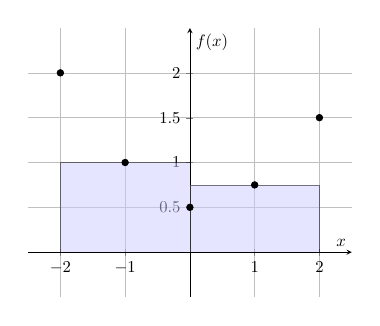
\begin{tikzpicture}[scale=0.6]
                    \begin{axis}[
                        axis lines = middle,
                        xlabel = $x$,
                        ylabel = $f(x)$,
                        xtick = {-2, -1, 0, 1, 2},
                        ytick = {0, 0.5, 1, 1.5, 2},
                        xmin = -2.5, xmax = 2.5,
                        ymin = -0.5, ymax = 2.5,
                        grid = both,
                        legend pos = north west
                    ]
                    \addplot[mark=*, only marks] coordinates {(-2,2) (-1,1) (0,0.5) (1,0.75) (2,1.5)};

                    % Fórmula del punto medio compuesta
                    \addplot[domain=-2:0, samples=2, fill=blue!20, opacity=0.5] {1} \closedcycle;
                    \addplot[domain=0:2, samples=2, fill=blue!20, opacity=0.5] {0.75} \closedcycle;
                    \end{axis}
                \end{tikzpicture}
                \caption{Pto. medio compuesta}
                \label{fig:ej2.1.17a}                
            \end{subfigure}
            \begin{subfigure}[b]{0.3\textwidth}
                \centering
                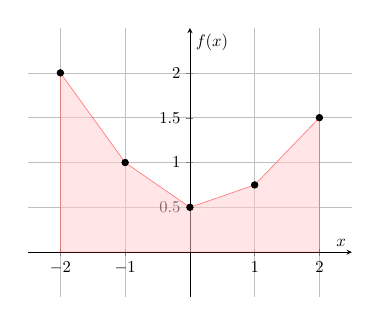
\begin{tikzpicture}[scale=0.6]
                    \begin{axis}[
                        axis lines = middle,
                        xlabel = $x$,
                        ylabel = $f(x)$,
                        xtick = {-2, -1, 0, 1, 2},
                        ytick = {0, 0.5, 1, 1.5, 2},
                        xmin = -2.5, xmax = 2.5,
                        ymin = -0.5, ymax = 2.5,
                        grid = both,
                        legend pos = north west
                    ]
                    \addplot[mark=*, only marks] coordinates {(-2,2) (-1,1) (0,0.5) (1,0.75) (2,1.5)};

                    % Fórmula del trapecio compuesta
                    \addplot[fill=red!20, draw=red, opacity=0.5] coordinates {
                        (-2,0) (-2,2) (-1,1) (0,0.5) (1,0.75) (2,1.5) (2,0)
                    } -- cycle;
                    \end{axis}
                \end{tikzpicture}
                \caption{Trapecio compuesta}
                \label{fig:ej2.1.17b}
            \end{subfigure}
            \begin{subfigure}[b]{0.3\textwidth}
                \centering
                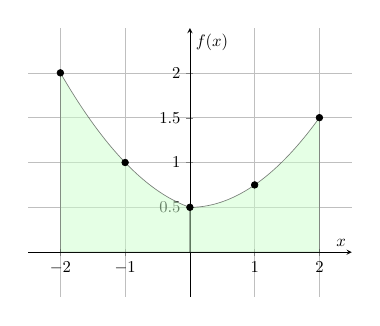
\begin{tikzpicture}[scale=0.6]
                    \begin{axis}[
                        axis lines = middle,
                        xlabel = $x$,
                        ylabel = $f(x)$,
                        xtick = {-2, -1, 0, 1, 2},
                        ytick = {0, 0.5, 1, 1.5, 2},
                        xmin = -2.5, xmax = 2.5,
                        ymin = -0.5, ymax = 2.5,
                        grid = both,
                        legend pos = north west
                    ]
                    \addplot[mark=*, only marks] coordinates {(-2,2) (-1,1) (0,0.5) (1,0.75) (2,1.5)};

                    % Fórmula de Simpson compuesta
                    \addplot[domain=-2:0, samples=100, fill=green!20, opacity=0.5] {0.25*x^2 - 0.25*x + 0.5} \closedcycle;
                    \addplot[domain=0:2, samples=100, fill=green!20, opacity=0.5] {0.25*x^2 + 0.5} \closedcycle;
                    \end{axis}
                \end{tikzpicture}
                \caption{Simpson compuesta}
                \label{fig:ej2.1.17c}
            \end{subfigure}
            \caption{Aproximaciones de $\int_{-2}^{2} f(x) dx$}
            \label{fig:ej2.1.17}
        \end{figure}
    \end{enumerate}
\end{ejercicio}

\begin{ejercicio}\label{ej:2.1.18}
    Calcule valores aproximados para $\ln 2 = \int_{1}^{2} \nicefrac{1}{x} dx$ usando las siguientes fórmulas y calcule una cota del valor absoluto del error que se comete en cada una de las aproximaciones obtenidas:
    \begin{enumerate}
        \item la fórmula del punto medio compuesta con 4 subintervalos,
        \item la fórmula del trapecio compuesta con 4 subintervalos,
        \item la fórmula de Simpson compuesta con 2 subintervalos.
    \end{enumerate}
    
    Compare los resultados obtenidos con los del problema \ref{ej:2.1.14}.
\end{ejercicio}

\begin{ejercicio}\label{ej:2.1.19}
    Se quiere calcular $\int_{0}^{1} e^{-x^2} dx$ usando la fórmula del punto medio compuesta. ¿Cuántos subintervalos deberá tener la partición uniforme a considerar para que el valor absoluto del error que se cometa al aproximar dicha integral sea menor que $5 \times 10^{-7}$?
\end{ejercicio}

\begin{ejercicio}\label{ej:2.1.20}
    Se quiere hallar un valor aproximado de $\int_{1}^{2} \ln^2(x) dx$.
    \begin{enumerate}
        \item ¿Cuántos subintervalos deberá tener la partición uniforme para que el valor absoluto del error que se cometa al aproximar dicha integral usando la fórmula del trapecio compuesta sea menor que $10^{-3}$?
        \item ¿Cuántos subintervalos deberá tener la partición uniforme para que el valor absoluto del error que se cometa al aproximar dicha integral utilizando la fórmula de Simpson compuesta sea menor que $10^{-3}$?
        \item ¿Cuál de las fórmulas compuestas de los apartados anteriores será preferible utilizar para aproximar la integral dada? Justifique la respuesta.
    \end{enumerate}
\end{ejercicio}

\begin{ejercicio}\label{ej:2.1.21}
    Se consideran las fórmulas simples del rectángulo, del punto medio, del trapecio y de Simpson. ¿Alguna de ellas es una fórmula de cuadratura gaussiana? Justifique la respuesta.
\end{ejercicio}

\begin{ejercicio}\label{ej:2.1.22}~
    \begin{enumerate}
        \item La fórmula numérica $f''(a) \approx \frac{3f(-2h) - 5f(0) + 2f(3h)}{15h^2}$:
        \begin{enumerate}
            \item ¿Es de tipo interpolatorio clásico?
            \item ¿Cuál es su grado de exactitud?
        \end{enumerate}
        \item ¿Existe alguna fórmula de derivación numérica, basada en $n + 1$ nodos distintos, de la forma $f''(a) \approx \alpha_0 f(x_0) + \alpha_1 f(x_1) + \cdots + \alpha_n f(x_n)$ que sea de tipo interpolatorio en $P_n$ y tenga grado de exactitud $n + 3$? Justifique la respuesta.
        \item Justifique que la fórmula de integración numérica $$\int_{0}^{2} f(x) dx = \frac{2}{3} (3f(0) + 3f'(0) + 2f''(0)) + R(f)$$ es de tipo interpolatorio en $P_2$ y para $f \in C^3[0, 2]$ su error se puede escribir como $R(f) = \frac{2}{3} f'''(\xi)$ con $\xi \in ]0, 2[$.
    \end{enumerate}
\end{ejercicio}

\begin{ejercicio}\label{ej:2.1.23}~
    \begin{enumerate}
        \item Calcule la fórmula de Gauss-Legendre con 2 nodos y halle la expresión de su error cuando $f \in C^4[-1, 1]$.
        \item Usando la fórmula del apartado anterior, obtenga una fórmula para aproximar $\int_{a}^{b} f(x) dx$ con $[a, b]$ un intervalo cualquiera. ¿Cuál es la expresión del error de dicha fórmula cuando $f$ es suficientemente regular?
    \end{enumerate}
\end{ejercicio}

\begin{ejercicio}\label{ej:2.1.24}
    Calcule la fórmula de Gauss-Legendre con 3 nodos y halle la expresión de su error cuando $f \in C^6[-1, 1]$.
\end{ejercicio}

\begin{ejercicio}\label{ej:2.1.25}
    Calcule la fórmula gaussiana con dos nodos de la forma $$\int_{-1}^{1} |x|f(x) dx \approx \alpha_0 f(x_0) + \alpha_1 f(x_1)$$ y halle la expresión de su error cuando $f \in C^4[-1, 1]$.
\end{ejercicio}

\begin{ejercicio}\label{ej:2.1.26}~
    \begin{enumerate}
        \item Determine los valores de $A$, $B$, $C$ de forma que la fórmula de cuadratura $\int_{0}^{3} f(x) dx \approx Af(0) + Bf(C)$ tenga el máximo grado de exactitud posible.
        \item Utilizando la fórmula obtenida en el apartado anterior, obtenga una fórmula para aproximar $\int_{a}^{b} f(x) dx$ con $[a, b]$ un intervalo cualquiera.
        \item Deduzca la fórmula de cuadratura compuesta asociada a la fórmula obtenida en el apartado anterior para una partición uniforme del intervalo de integración $[a, b]$ en $N$ subintervalos.
    \end{enumerate}
\end{ejercicio}

\begin{ejercicio}\label{ej:2.1.27}
    Halle la fórmula de cuadratura de la forma $\int_{-1}^{1} f(x) dx \approx \alpha_0 f(-1) + \alpha_1 f(x_1) + \alpha_2 f(1)$ que tiene el máximo grado de exactitud posible. ¿Cuál es ese grado de exactitud máximo? ¿Se trata de una fórmula de cuadratura gaussiana? ¿Por qué?
\end{ejercicio}

\begin{ejercicio}\label{ej:2.1.28} Las fórmulas gaussianas de Laguerre corresponden a una integral del tipo
    \begin{equation*}
        \int_{0}^{\infty} e^{-x} f(x) dx.
    \end{equation*}
    \begin{enumerate}
        \item Obtenga la fórmula de Laguerre con dos nodos.
        \item Aplique la fórmula obtenida para aproximar $\int_{0}^{\infty} e^{-x} x^4 dx$.
    \end{enumerate}
\end{ejercicio}

\begin{ejercicio}\label{ej:2.1.29}
    Se denominan fórmulas de integración de Lobatto a aquellas que usan como nodos los dos extremos del intervalo de integración, y eligen los restantes para alcanzar la máxima exactitud posible. Trapecio y Simpson son ejemplos de fórmulas de Lobatto, siendo la del trapecio la más sencilla.
    \begin{enumerate}
        \item Obtenga la fórmula de Lobatto del tipo $$\int_{-1}^{1} f(x) dx \approx \alpha_0 f(-1) + \alpha_1 f(x_1) + \alpha_2 f(x_2) + \alpha_3 f(1)$$
        \item Obtenga la expresión del error de dicha fórmula.
    \end{enumerate}
\end{ejercicio}

\begin{ejercicio}\label{ej:2.1.30}
    Se necesita calcular $$\int_{0}^{1} x f(x) dx \approx \alpha_0 f(x_0) + \alpha_1 f(x_1)$$ Obtenga $x_0$, $x_1$, $\alpha_0$, $\alpha_1$ para que la fórmula anterior tenga exactitud máxima.
\end{ejercicio}